Workshops today!

\subsection{Workshop: AI for Climate Change}

First, John Platt (a follow up to his wonderful talk a few years back!)

\subsubsection{John Platt on What ML can do to help Climate Change}

\dbox{{\bf Main Point:} Energy research is not the same as fighting climate change.}

$\ra$ Climate crisis: we are running out of our carbon budget! Without intervention, our best models project \\

Turns out we can't stop energy infrastructure (trillions invested). Best we can do is slowly stop using them: might achieve a 3\% reduction (in energy use), or if we suppose some {\it miraculous} rate, maybe 10\%.\\

$\ra$ Assuming {\it rapid decarbonization} (of 10\%), in order to hit our goal (as defined by the Paris agreement), we have to start {\bf now}! \\

$\ra$ Okay, but what if it's not radical? More conservative: 3.3\%.

Measure: Final temperature rise ($^\circ$).

{\bf What needs to Happen?}:
\begin{itemize}
    \item Decarobize rapidly and quickly to avoid >$2^\circ$.
    \item Zero carbon energy technologies must be shovel ready
    
    $\ra$ Renewables are ready now, relatively scalable.
    
    \item Post 2040 zero carbon technologies still useful.
    $\ra$Backstop to avoid absolute worst climate change
    
    $\ra$ Scenario of plentiful energy for everyone still achievable and desirable.
    
    
\end{itemize}


{\bf Idea:} Suppose we want to deploy renewable energy tech (solar, win, and so on). \\

$\ra$ Problem: Demand and supply fluctuate dramatically, and thus there will likely be gaps between when we have energy and need energy (consider a cloudy day!).\\

Code/work available exploring cost of renewables called DOSCOE~\cite{platt2017analyzing}. Code: \url{bit.ly/DOSCOE}. \\

Q: Can ML help this problem?
\begin{itemize}
    \item Most valuable zero-carbon sources are dispatachable (like hydropower)
    \item Can dispatch demand as well (turn on when carbon intensity of supply is low)
    \item Can ML/aI demand response?
    $\ra$ Google  reported 40\% less energy spent on data center cooling via ML control.
\end{itemize}

Two Caveats:
\begin{enumerate}
    \item Many sources contribute to climate crisis. Breakdown from John's ``pie-chart of sadness": Industry: 21\%, Electricity and Heat production 25\%, Transportation: 14\%, Buildings 6\%, Agriculture/Forest and other Land use: 24\%.
    
    \item Require ``carbon pressure": the free market doesn't encourage these practices!
    \begin{itemize}
        \item Currently no incentive for demand response
        \item Increased efficiency lowers price of electricity and fossil fuel
        \item Less energy use $\ra$ more income + economic growth $\ra$ more energy.
        \item Efficiency makes people better off, even with Jevon's paradox (save 1J of energy, cause >1J of energy consumption).
    \end{itemize}
\end{enumerate}

{\bf Idea:} ML for material science? 1) New ways of making concrete?, 2) Fixing nitrogen?, 3) Better batteries?, 4) Neutron-resistant materials? \\

$\ra$ Other ideas: detect methane leaks (w/ ML)? Telepresence to reduce transportation (notably a very high bar)? Optimize freight?\\

Other things ML can do to help:
\begin{enumerate}
    \item Flood forecasting:
    \begin{itemize}
        \item Floods are bad now: 9.8 billion annual damage, effects 250 people per year
        \item Will get worse at higher temperature!
        \item Goal: forecast flood effects using public data.
        
        $\ra$ Problems: data usually too noisy, floods usually in flat areas.
        
        \item One solution: use ML to derive surface maps, can be used to forcase more accurately
    \end{itemize}
    \item Moonshot: push C02 out of atmosphere in second half of the century.
    \begin{itemize}
        \item Bio-energy with carbon capture and sequestration (already assumed in IPCC pathways).
        \item Increase carbon in soil via plants (soil contains $>3\times$ carbon of atmosphere)
        \item Free air capture (David Keith claims \$100 per ton cost).
        \item Can ML/AI help any of these?
    \end{itemize}
\end{enumerate}


{\bf Summary:}
\begin{enumerate}
    \item Climate and energy is a huge problem
    \item Major takeaway: multiple time scales
        1) ML/AI can help long term technologies (post 2040)
        2) But, need immediate and radical carbonization now.
    \item Many sources/sinks of greenhouse gases. But, no single silver bullet, must push on many fronts at once.
    \item No purely technological solution.
\end{enumerate}


{\bf Call to Action:}
\begin{enumerate}
    \item Find an ML application (get inspiration from recent paper)
    \item Collaborate with domain experts, and 3) Start work and don't settle!
    \item Don't be satisfied with saving 10,000 tons of CO$_2$.
    $\ra$ This a huge problem: aim for megatons!

    $\ra$ Also: massively hard problem. Most things don't work.
\end{enumerate}

\spacerule

\subsubsection{Jack Kelly: Why It's Hard to Mitigate Climate Change, and How to Do Better}

{\bf Goal:} Help us reduce emissions as rapidly as possible. \\

\dbox{{\bf Central Question:} Why is it hard to reduce carbon emissions?}

Visual: industry on the left, a ``mountain of pain" in the middle", researchers and start ups on the right. What is this mountain, and how can we mitigate it? \\

Jack recently founded Open Climate Fix, a non-profit based on two hunches:
\begin{enumerate}
    \item Open science, share data, help researchers and companies be successful in their endeavors on fighting climate change,
    \item Develop better forecasting tools for helping predict the amount of available solar energy.
    
    $\ra$ Developing an open platform of solar panels in the world. With better forecasts, less spinning reserves.
\end{enumerate}

{\bf Challenges:}
\begin{enumerate}
    \item {\it Incentives:} Wrong incentives in the world---companies optimized to maximize profit, scientists optimize h-index, neither of which well align with climate challenges.
    \item {\it Data:} Lots of challenges here:
    \begin{enumerate}
        \item 1) organizations reluctant to share (companies believe it has commercial value, data the new oil, etc), 
        \item Size
        \item Under diagnosed systems
        \item Quality: often extremely noisy, missing labels, and so on.
        \item Access: sometimes in different/unusual physical forms, no standardization.
        \item No perfect simulators.
    \end{enumerate}
    
    But, some solutions: 1) Budget lots of time for data engineering! 2) Ask questions early, 3) Find people who can help, 4) Be flexible, and 5) Use simple models.
    
    \item {\it Intellectual Property:} Most things are behind closed doors. \\
    
    $\ra$ But, some solutions: 1) Open source everything, 2) Talk to commercialization teams (universities/labs).
    
    \item {\it Industry is unlikely to read your paper:} You need to sit down with people in industry and work on their problems. Help industry use your algorithm! Build a production service, consult, and so on.
    
    \item {\it Demonstrating Performance:} No standard datasets or metrics or benchmarks.

    
\end{enumerate}


{\bf Takeaways:}
\begin{enumerate}
    \item Spend as much time as possible with people in the industry you're targeting.
    \item Be lean, build a minimum viable product, rapidly test your ideas. Fail, and fail fast, then move on to the next thing.
\end{enumerate}

Audience Question: Can you mention why it's so useful to spend time with industry folks? Any specifics? \\

Jack A: Sure! Great point. Consider working with forecasting clouds. One thing we'll need to do is estimate the 3d structure of clouds. It's hard but with conversations with the meteorologists we can estimate volumetric info from rain fall and numerical weather predictions. Super valuable talking to industry folks, couldn't imagine doing this online. \\

Audience Question: Do you think a carbon tax could be better communicated to put it in motion? \\

Jack: Great question! Maybe we need to change the term (people don't like the term ``tax"). Figuring out a better way to communicate such things is really important.

\spacerule

\subsubsection{Andrew Ng: Tackling Climate Change with AI through Collaboration}

{\bf Backdrop:} We have already seen massive impacts from climate change (see: more fires, flooding, and other disasters). \\

$\ra$ Many of our children will be alive in 2100. The decisions we make today will directly shape the world they live in. \\

Lots to do: 1) Mitigation (energy, industry, buildings, forest), 2) Adaptation (disaster prevention, societal/ecological) 3) Alteration (sequestration), 4) Climate Science. \\

{\bf Project One:} Methane prediction (second most important greenhouse gas).
\begin{itemize}
    \item Methane comes 50/50 from human and natural sources.
    \item Biggest source of methane source are {\it wetlands}.
    \item Unlike CO2: Limited number of sensors around the world to detect methane.
    
    $\ra$ Andrew and colleagues visited a methane sensor: every few weeks, one of the researchers has to visit the sensor to collect data.
    \item Ng et al. now have access to 37 methane sensors around the world.
    
    {\bf Idea:} Use these data to then predict methane emissions elsewhere in the world! Using data from these sensors, can now predict methane all over the world.
\end{itemize}

{\bf Project Two:} Wind turbine detection
\begin{itemize}
    \item The world is moving toward renewables
    \item But, a problem: with the way solar and wind farms are rolled out, we don't often know where they are.
    
    $\ra$ To facilitate growth and integration of renewables, we need to {\it locate} renewables.
    
    \item Can improve USGS database of renewable location by: 1) automatic curation, 2) updating frequently.
    
    \item To locate wind turbines:
    \begin{itemize}
        \item Data consisting of 100k images of locations of wind turbines.
        \item Run detection on 1.8M images
        \item Baseline model: DenseNet-121
        \item Weakly supervised localization: GradCAM.
    \end{itemize}
    \item {\it Estimating Wind Energy:} With these models, have a good estimate of location of wind turbines {\it and} a good estimate of wind in the US (see: \url{http://hint.fm/wind/}).
    
    $\ra$ Combined with their work, DeepWind, can then predict energy output of wind turbines in the USA.
\end{itemize}

{\bf Other Projects:} 
\begin{itemize}
    \item Machine learning for Modeling Atmospheric Convection~\cite{o2018using}
    \item Spatiotemporal Global Climate Model Tracking
    \item Mitigation: optimizing renewables. DeepMind predicts wind power output 36 hours ahead of schedule.
    \item GasNet: using deep learning to automatically detect methane leaks from real-time videos at natural gas power plants~\cite{wang2019machine}.
    \item Economic Impact: better understanding of how climate change will impact economically different countries ~\cite{diffenbaugh2019global}.
\end{itemize}

Echoing Jack's point: we need to collaborate with climate scientists, ecologists, meteorologists, and so on! See Figure~\ref{fig:venn}.

\begin{figure}
    \centering
    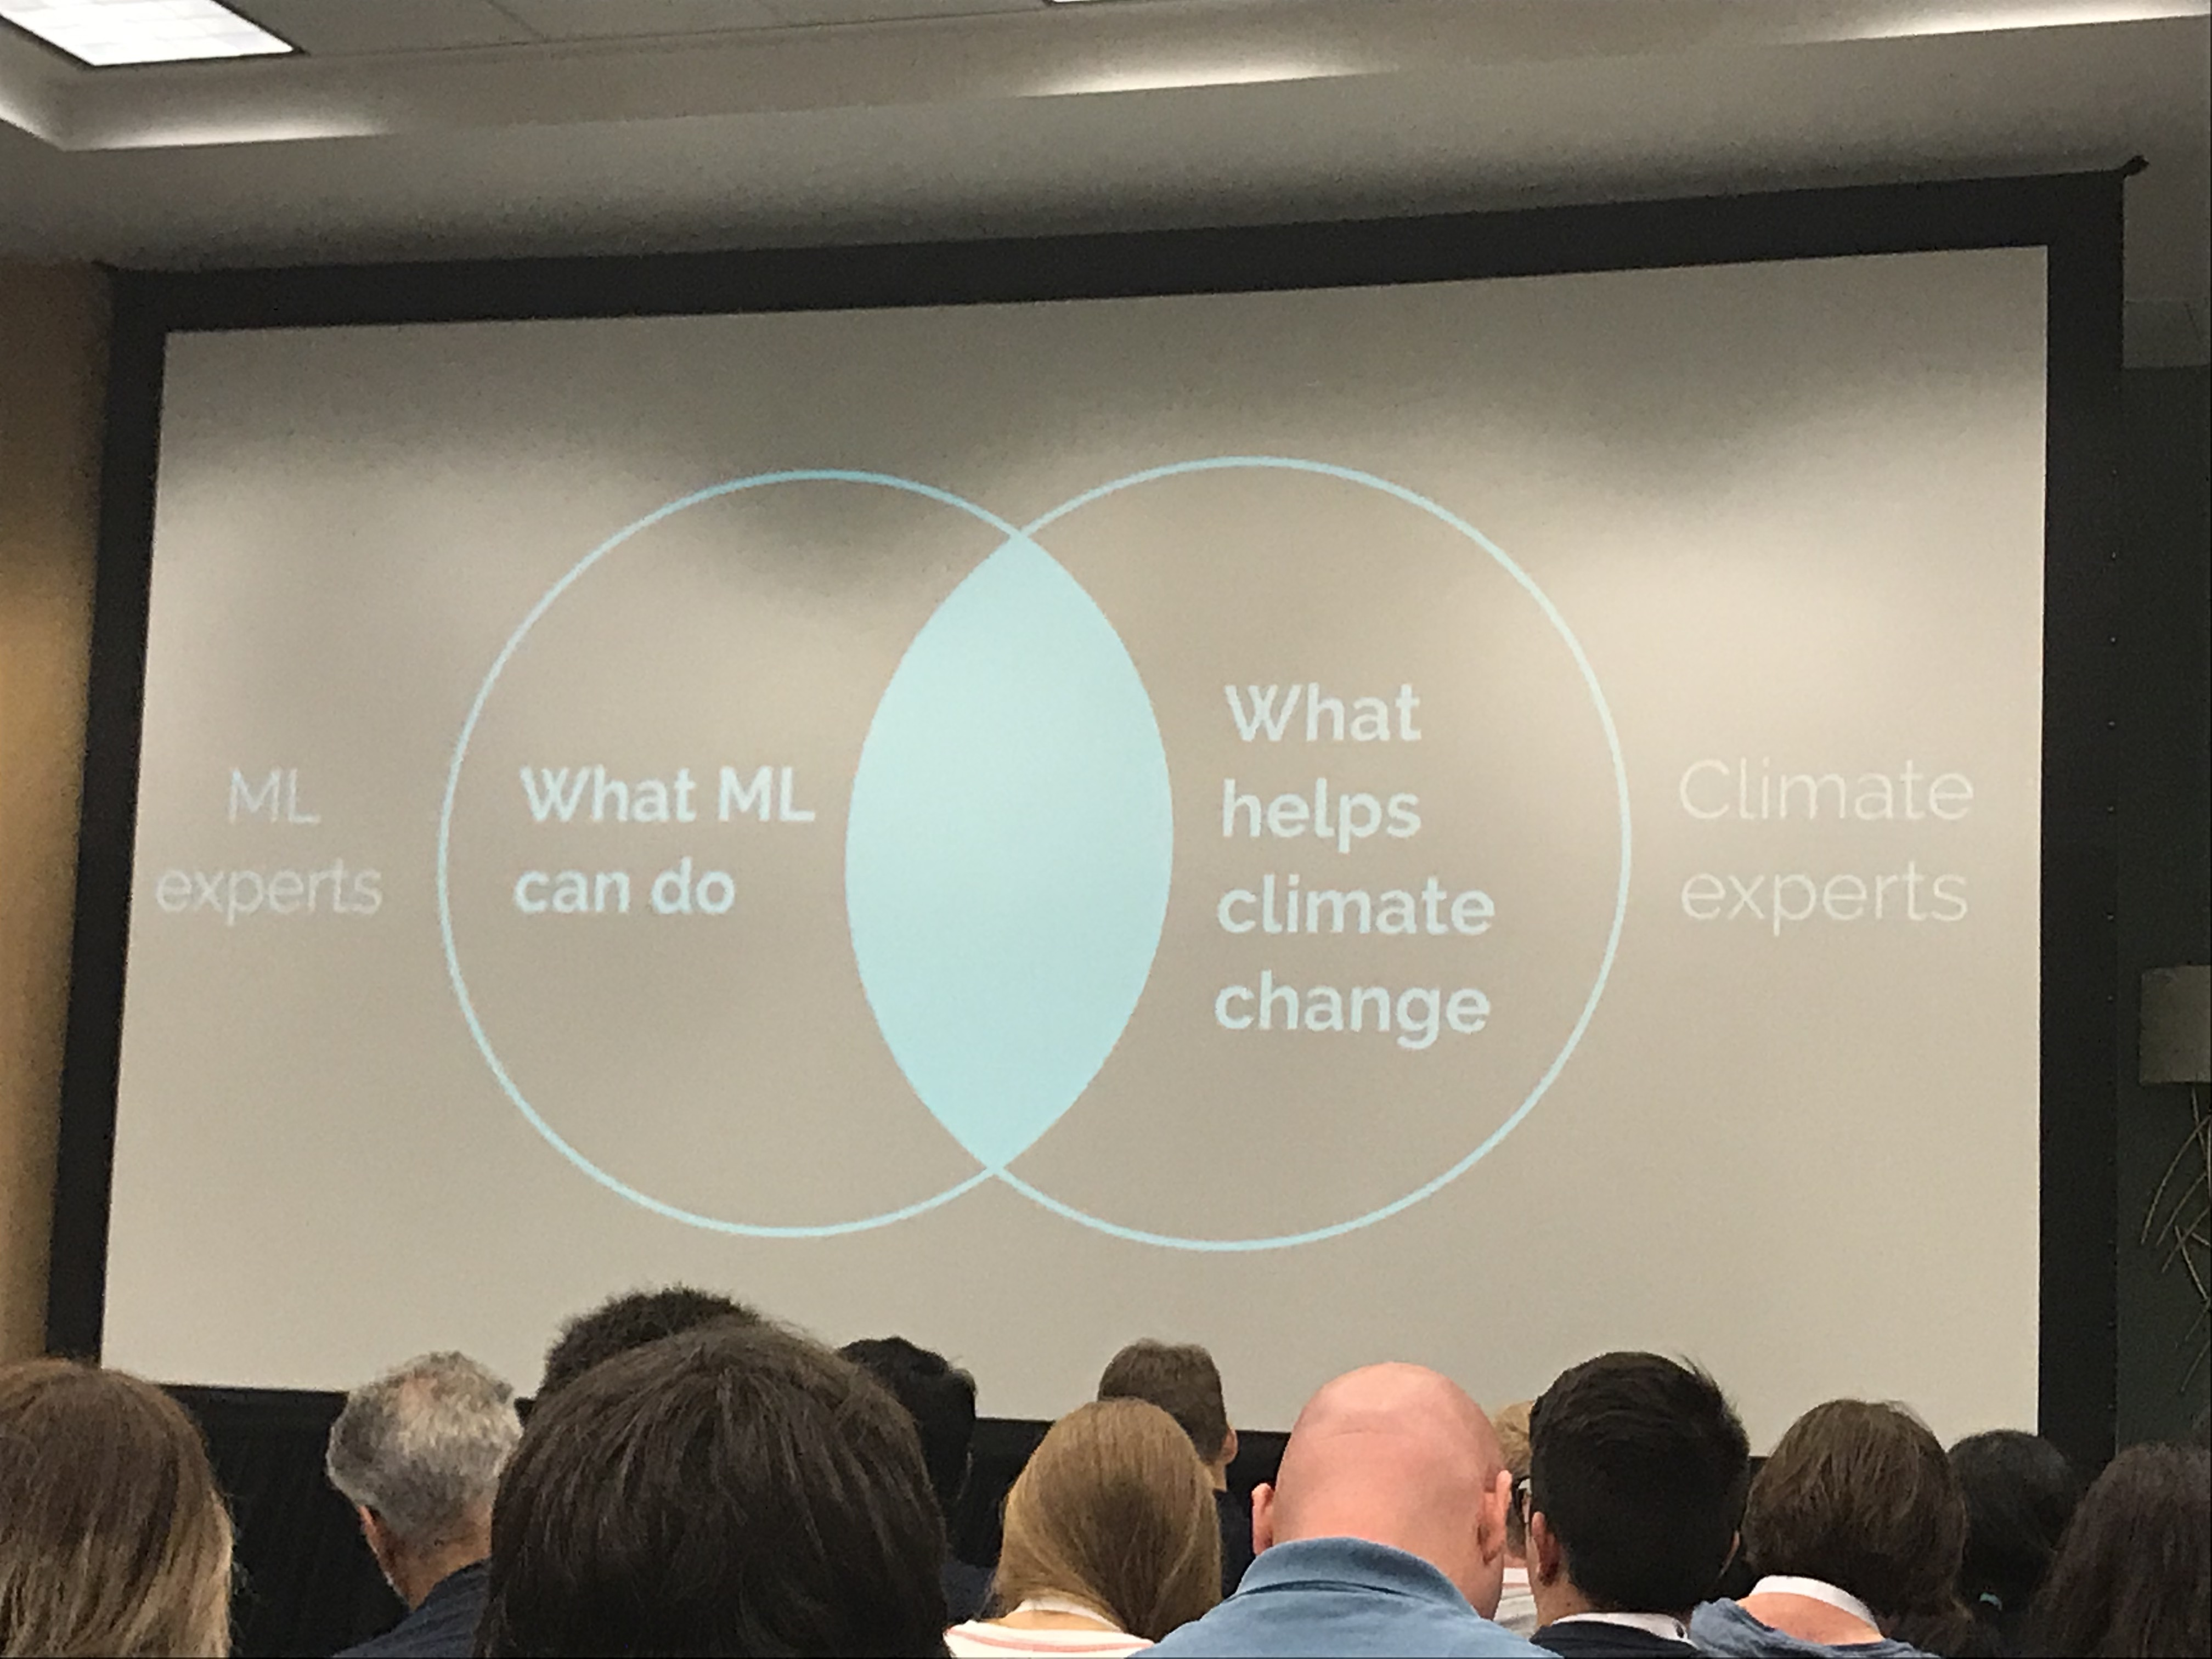
\includegraphics[width=0.5\textwidth]{images/venn.JPG}
    \caption{Call for collaboration across ML and climate science.}
    \label{fig:venn}
\end{figure}


{\bf Concluding thought}: In eras of technological disruption, collaboration matters. Work together! Share data! This problem is bigger than ourselves.

\spacerule

\subsection{Workshop: RL for Real Life}

I arrived just in time for the panel.

\subsubsection{Panel Discussion}
\label{sec:panel}

The panelists are Craig Boutilier (CB), Emma Brunskill (EB), Chelsea Finn, Mohammad Ghavamzadeh, John Langford, David Silver, and Peter Stone. I'll abbreviate each by their initials. \\

Moderated by Alborz Geramifard (AG). \\

Q: What application areas are most promising for RL and why? \\

JL: Bread and butter baseline is personalization---of news stories, of advice, layouts, many other things. \\

CB: For me, interested in agents that can act on behalf of users, lots of problems though (multi-agent, preference elicitation). Recommender systems are promising but also challenging. We won't see wins short term, but recommender systems long term over long periods of time should serve as a really valuable test bed and a way to stress RL algorithms. \\

PS: We need a definition of promising to answer the question. Excited about promise of RL in robotics and manipulation, like my colleagues, the general class of user engagement through nudges/influencing people's behaviors in helpful ways (insidious ways, too, though). Help people rehab or take medicine; well fit for RL. We do have to think about what settings in the real world are safe/well fit. \\

CF: The best fits for RL are not really the problem the community focuses on. MuJoCo for instance has served its purpose for a time, but we need to scale now to partial observability, transfer, continuous state/action. Robotics fits that well though. \\

JL: Moving beyond bread and butter that are deployed right now, I think system optimization is a natural area for RL application. Most of these systems have a good recording over time, so lots of data (and don't have to wrestle with uncertainty). \\

EB: Personalization is a raw term, lots of things are changing in the world. Prior applications (when I was in grad school) was robotics and games. Opportunities now for personalization, given the world right now, is both a huge responsibility {\it and} exciting opportunity. \\

DS: Follow up to something John said in his talk---if we get the foundations right, there will be applications everywhere. If we get an algorithm that just works, we should expect to see RL in all kinds of places. Who knows what methods/approaches are out there? Let's continue to push the foundations. We should of course keep pushing and try to deploy it too, but I think we can expect to be surprised too. Looking a little farther in the future, one open area where there's huge potential for getting RL right is personalized healthcare. Can transform many peoeple's lives. \\

MG: Lots of OR applications everywhere---think about system optimization, huge opportunity for RL. What's happening with Amazon storage facilities. One more thing for recommendation systems. Recommender systems are everywhere and we have tons of data. Consequences of our actions are clear, need to consider safety and robustness. Although consequences of actions in recommender systems aren't catastrophic, it's still important we get it right. \\

\spacerule

AG Q: Great segue into next question. How should we explore in these problems? \\

DS: Part of every framework, even in simulation. We always have to handle explorations (agents die, we don't receive more reward/data). If it has opportunity to come back and learn more, then we can still learn from the {\it lack of experience} to get more. That's nice in recommender systems too since we get ``parallel lifetimes", if a stream of experience stops we can still learn from it. It's signal that someone stopped using the system \\

CB: Yeah except for people that die in certain trajectories. Maybe not in recommender systems but in broad multi-user systems. In multi-user systems you get to distribute these decisions/explore. Can learn from individual users in a distributed way to guarantee safety (no individual action that can be so bad). In clinical setting, in recommender setting, can distribute exploration to not do damage to any individual. \\

EB: I think this is a really interesting question in a lot of settings---it's a reason to use policy gradients or imitation learning or methods with monotonic improvement. Some work shows we can be optimal too (be greedy w.r.t. information we have so far can still do well). These kinds of approaches help us avoid the major burdens of exploration. Lots of tools and directions to make progress. \\

PS: To me it's a fascinating question of meta-learning. When we do have a big population of users, should we pick a small subset and burn them and use our exploration budget, or should we explore a bit across all users (or other strategies)? Meta-objective: keep population happy with what you're doing, so: how should we achieve this? \\

CB: Quick response. If we have a model of cost of exploration this all falls out of the wash.\\

JL: This is a place where theory is really important. If we're going to optimize only for efficiency, you'll be driven away from $\eps$-greedy, and if we want to think about safety, we can use bounds to guide decision making in a safe way. \\

MG: Ways to make exploration more conservative. How conservative can we be? Well that depends on individual task/product/setting. If we know information about users/domain, we can set the exploration appropriately. Another important question: how do we fill the gap between simulation and the real world? Really hard. But having those simulators will help us explore in the world. \\

DS: Even in the real world, there are times when users leave, and we can actually continue to learn from these settings. If we do it right, it's all there in the framework: how should we maximize reward? Sometimes we take actions that keep people engaged or not, and that's ok. \\

EB: One thing we've been thinking about is how to keep exploration safe. Idea: policy certificates. Can promise explicitly how a particular method will explore/behave. We can have tools that can allow us to expose when we're going to explore and when we won't.

\spacerule

AG-Q: What are general principles that are key for bringing RL to the real world? \\

JL: First principle is that the framing of the problem is more important than anything else. Second one: if I gave you a long laundry list of things that are more important in real world than simulated worlds. \\

CF: One principle important to safety is to {\it identify} cases where it's safe to explore. Maybe you buy a small robot first and then transfer what it learns (like it's okay to fall down as a kid to learn from it). Identify situations where it's safe to explore, then can maybe be equipped to explore in new situations. \\

PS: Biggest lesson---simulators are never perfect! Super appealing because they're safe and we can get lots of data. We should use simulators, but we're never going to get them perfect. Efforts to make simulators perfect are misguided we should make new methods. \\

CF: Completely agreed! If you could make a simulator that's perfect you've already solved the problem. Learning in the real world is going to be required. \\

CB: One other principle I'd like to raise---reward function and objective function design. That first reward function you specify is never the right one! We walk away and say ``this is the best policy", but it's clearly not based on the behavior, we got the reward function wrong. Human-in-the loop methods are really important for correcting/designing the right objectives/reward functions. \\

EB: I want to echo that---my lab does a lot of work in education and healthcare. Coupling this work (and these choices of reward functions) with domain experts is massively important. The first known application of RL to education was in 1999 to understand how students do well on problems. Example: give students problems until student gets it right, then give the student the same one over and over again (exploit!). \\

DS: Number one principle in my own work---scalability. We should only try to strive for methods that scale well with resources (three: 1) compute, 2) experience, 3) memory). If we can achieve that level of scalability, we just need to scale up the resources. If we design something where we put a ceiling into the method itself (stop exploring, stop learning, other constraints), that ceiling will hurt us. Goal should always be scalability.  If you look at the success of deep learning, I claim it's successful because it scales with all three things (compute, experience, memory). It does better and better with these resources. So we should find the RL methods that scale. \\

MG: First principle is to make sure RL is the right solution for your problem. Second, make sure we have the data available for RL. Think about supervised learned, if half your data is bad, you can still do well. Same situation for RL we can't do well. Reiterate what Craig said: reward functions are super important. Part of the reward function might be company profit (as opposed to say, customer happiness). \\

JL: I want to mention I agree with David. The process of educating people on the realies of RL is always fun. \\

PS: The design principle of our platform at Cogitai is a two part hypothesis: 1) RL is ready for the real world (that is, we, in this room, are ready to solve problems in the real world), and 2) the real world is ready for RL. This second piece is what John mentioned. Lots of problems in the world we know RL is ready, but it's a big challenge for us to work with folks from outside RL/ML to help them identify which problems are RL problems and help them use RL tools to solve their problems. The first bucket is easy (us find RL problems) while the second is hard (convince others). Important point from David: we're going to be surprised! It wasn't the people that made the smartphone that built the apps. We build the technology and tools that enable people outside this room to use these ideas. That's the goal. Get it robust enough that we can be surprised. \\

CB: Widespread acceptance of RL is ultimately an important goal. We could have been having this same conversation $N$ years ago about ML in industry. Not very long ago just getting ML to be accepted in large scale production systems, but here we are. \\

\spacerule 

Audience-Q: (paraphrased by PS): can we compare approaches to supervised learning and RL on real problems? \\

PS: Well, I don't think it's well posed to do this test. There are RL problems and supervised problems. These are different. \\

JL: Consider recommendation. Enormous number of actions. To apply RL to an enormous number of things often won't work. If you have a supervised signal source, that doesn't suffer from same sample complexity issue. Could apply RL on top to get the personalization which you can't really get from SL. There is no representational limit to RL---the same representations that can work for SL can work for RL. We've done reductions between these and this works. \\

CB: You can treat RL problems as supervised learning problems in recommender systems. Make a prediction, store it. The differences is whether we're being myopic vs. looking at the long term. The question is, if you learn representations about how users act in long term vs. short term, do you get some benefit? I don't know. \\

DS: A comment about A-B testing. You raised it as if it were outside RL, but you can think about it as a bad RL algorithm. Do this one thing and stick to it, do this other thing, then compare how these do after the trial. That's part of RL but we can also do better like contextual bandits. \\

\spacerule

Audience-Q: On horizons/reward design. Algorithms might exploit human weaknesses more heavily in the future, a lot of the behaviors of ML algorithms are probably due to their mmyopic nature. Being able to look ahead for multiple timesteps might allow for better reward functions. Thoughts? Second, when we use RL for problems with humans in the loop, what is the longest horizon we can actually use. \\

JL: Right now, typically, horizon is relatively short (hours, minutes, days). As that increases data is harder to come by. If we succeed in RL there's no reason it can't be lifetimes. \\

EB: Depends on what level of granularity you're using: hierarchical can help here! Both of those views are definitely possible. The technology we're developing is dual use and an amplifier. Will be constrained by the people and not the techniques themselves. \\

CB: Totally agree with with John and Emma. I still don't think we have the technology in our hands to do multi-scale planning, but we'll get there. With respect to doing right by the user. One important thing: we really don't have good methods for understanding user preferences and utilities, and how their behaviours reveal these. Real limiting factor to applying RL over long horizons is a developing techniques where we can know quickly what a users' utility function is. RL is also about planning but we're far from being able to do that.

CF: On reward design and David's comment about scalability---we should be thinking about algorithms that scale, but if we're in the real world, reward function supervision isn't a scalable source of feedback. In those settings is important to consider how we should frame the problem so it's scalable. Shouldn't be afraid to change the problem statement. For example, if you want a scalable algorithm, design a setting and algorithm that can scale with the resources involved. Don't really feel constrained by the classical RL statement if your problem doesn't match that.

\spacerule

Audience-Q: First, when is a policy safe to deploy? \\

PS: Tempting but wrong: Deploy when optimal! Will definitely depend on domain. Testing should be empirical---can we drive better than people? \\

EB: Can learn a lot by looking at verification (in RL, in deep learning). For these examples, sometimes people can't be in the loop to verify. Can use these to avoid worst-case scenarios (see: making aircrafts avoid collisions). Some safety guarantees. \\

JL: Practical answer: frame your problem so no actions are particularly bad/catastrophic. Then do RL on top of that.




PS: RL has components that are Art and components that are Science. We've been trying to make it 100\% science, but we need to accept that parts of it are art.

\spacerule


{\it Lihong Li on closing remarks:} 
\begin{itemize}
    \item Goal of workshop: Bring together researchers and practitioners from industry and academia interested in addressing practical and/or theoretical issues in applying RL to real life scenarios. 
    \item RL in real life: games, robotics, transportation, resource allocation.
    \item Challenges: partial observability, multi-agent systems, stochasticity, large action set, simulators, evaluation, generalization.
    \item Post workshop discussion via slack (on the workshop website: \url{https://sites.google.com/view/RL4RealLife}).
\end{itemize}


\spacerule

Next up is the afternoon session of a closely related workshop.

\subsection{Workshop: Real World Sequential Decision Making}
\label{sec:off_pol}

The workshop begins with an invited talk by Emma Brunskill.

\subsubsection{Emma Brunskill on Efficient RL When Data is Costly}

{\bf Questions:} What's the best way to teach a student coding? How should this patient be treated for cancer? Will job training increase future income? \\

$\ra$ We'd like to answer these question in an evidence based way! See: interventional science. \\

{\bf Problem:} The way we do interventional science at the moment is flawed. Example: run a bootcamp. See which intervention leads to higher graduation rates. One idea: dynamically adapt how we assign students to conditions. $\implies$ use RL! \\

$\ra$ Can use RL to understand the science of intervention. \\

Historical test beds: video games and robots. Now, though: new kinds of test beds. \\

Recent changes: massive compute, massive sensors, and ability to dynamically interact with people. 

$\therefore$ opportunities to apply RL have emerged! Lots of negatives to this, but many opportunities too. \\

{\bf Goal:} Learn to make good decisions faster (in a statistically efficient way), to benefit more people. \\

Q: How can we create AI that help students? \\

A: Project---RL assistance leads to 1.3$\times$ faster learning, longer learning, and more learning. \\

Key Techniques:
\begin{enumerate}
    \item Exploration!
    \item Counterfactual/Batch Off Policy RL (focus today).
    
    $\ra$ Tension between beautiful math and impacting society. But! This area allows for both.
    
    $\ra$ Growing interest in Causal Inference and ML. See: {\it The Book of Why} by~\citet{pearl2018book}.
\end{enumerate}

Q: How can we learn from historical sequential data? \\

A: It's really hard! Many challenges: data generation process is fundamentally different. That is:
\[
\tx{Different Policies} \implies \tx{Different Actions} \implies \tx{Different States}
\]
That is: decisions {\it compound}. \\

$\ra$ Moreover: we don't even know the behavioral policy. \\

{\bf Classic challenge:} Batch Off Policy Evaluation. We're given a dataset $D$ of trajectories gathered by some policy $\pi_D$, and we would like to compute the value of some new policy $\pi'$. \\

$\ra$ One spin: batch off policy {\it optimization}. Just want to know how to {\it act}, given data from prior policy. \\

Example: when should we treat patients? Really, how can we come up with a {\it personalized} policy for when to intervene (take a ventilator off, for instance). \\

$\ra$ One specific kind of intervention policy: vast majority of decisions are ``nothing", then suddenly we have to intervene. Let's call such a decision the \texttt{when-to-treat-policy}. \\

Q: When should we start HIV treatment? When should we stop some kind of treatment? \\

$\ra$ These cases are well captured by parameterized policies conditioned on relevant contexts. \\

Two solutions: Importance weighting (also called ``inverse propensity weighting"). Goal is to estimate expected value of new \texttt{when-to-treat-policy}. \\

$\ra$ Advantage: simple and consistent
$\ra$ But: uses only trajectories that match data, not very robust, high variance. \\

{\bf New Idea:} Advantage decomposition: $\tau_\pi$ is a stopping time w.r.t. some filtration \texttt{when-to-start-treatment} according to policy $\pi$. Then:
\begin{align}
\mu_{now}(S_{1:t}) &= \bE\left[\tx{Return}\right] \\
\mu_{next}(S_{1:t}) &= \bE\left[\tx{Return}\right]
\end{align}
If we can determine which $\Delta_\pi := V^\pi - V^{\pi_0}$, where $\pi_0$ is the \texttt{never-treat} policy, we can determine the advantage of a particular treatment. \\

$\ra$ Specifically: want to estimate $\Delta_\pi$ from data, even {\it without} $\pi$. \\

Yields the {\bf Advantage Double Robust} (ADR) Estimator for off policy evaluation in the when to treat context. Yields regret bounds, too. Further differences visualized in Figure~\ref{fig:off_policy}.

\begin{figure}
    \centering
    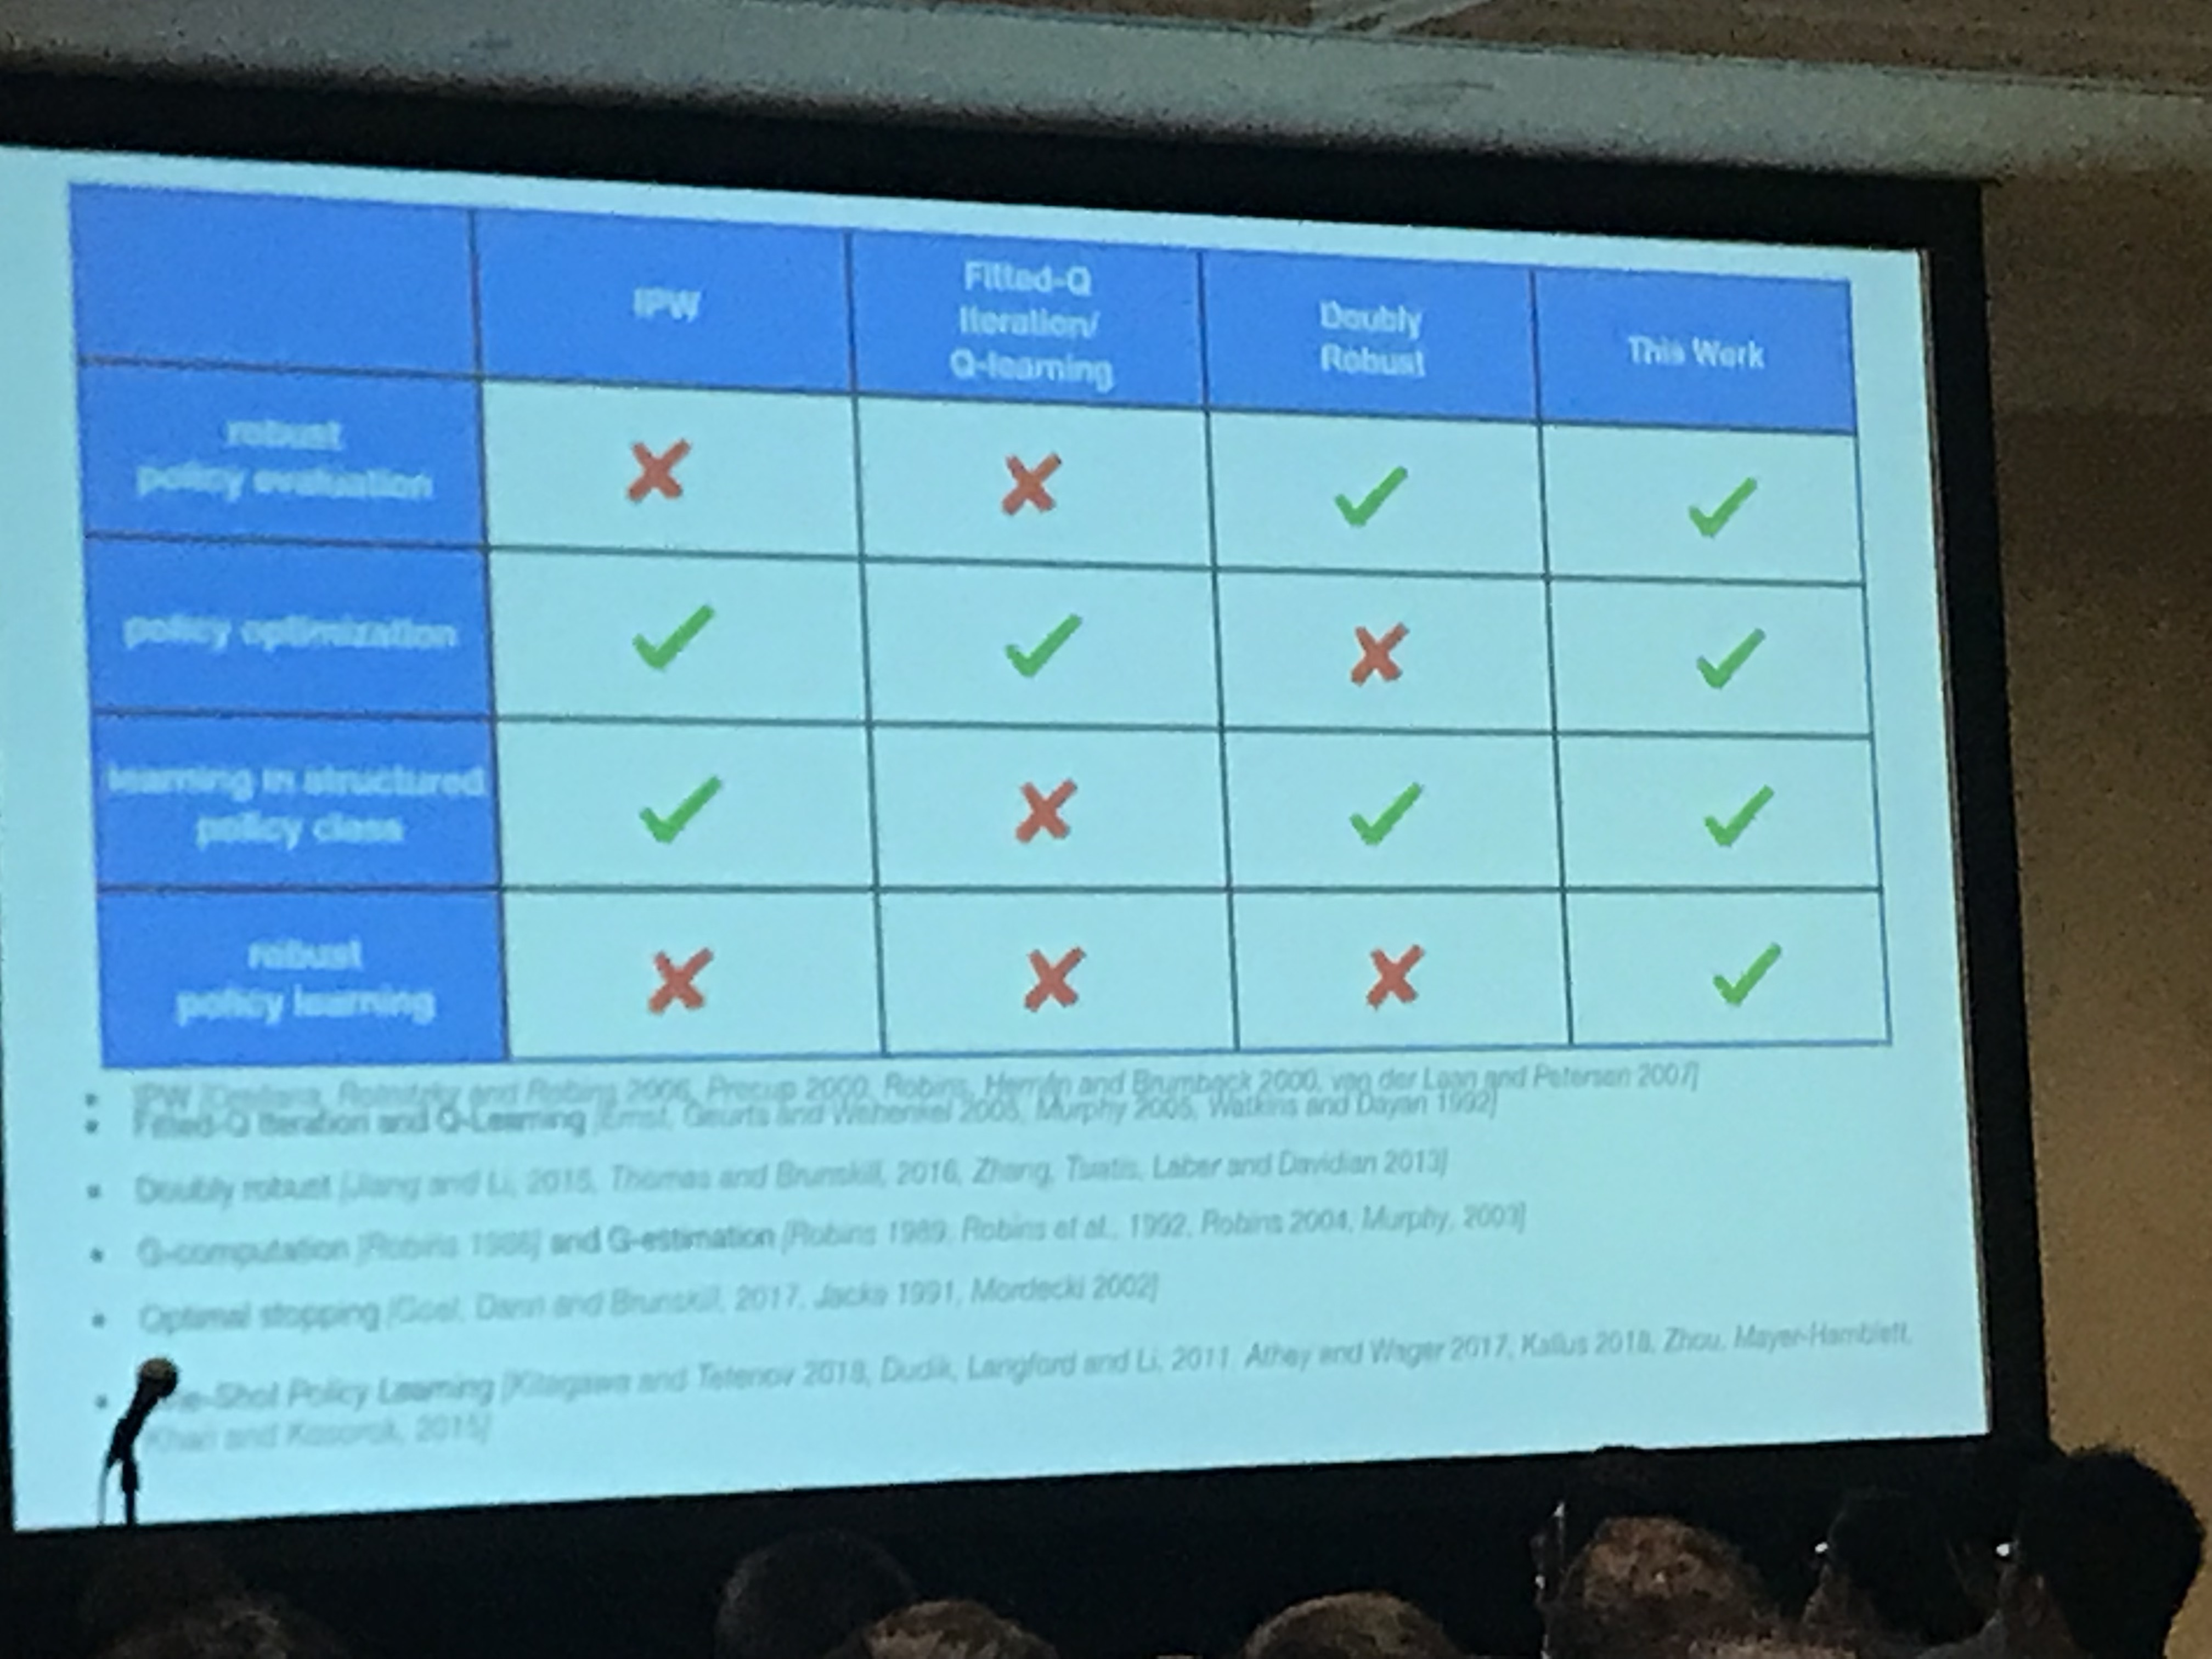
\includegraphics[width=0.5\textwidth]{images/off_pol.JPG}
    \caption{Comparison of different off-policy evaluation types.}
    \label{fig:off_policy}
\end{figure}

{\bf Experiments:} Keeping a health metric above 0, where state evolves over time in a stochastic way (with brownian motion). Use treatments to try to help outcomes. \\

$\ra$ Given observational data from clinic, want to find way to choose effective treatments. \\

Another important question: how can we estimate $V^*$? (perhaps, specifically to help human-in-the-loop)\\

Q: Can we identify with $< O (d)$ samples if there exists a linear threshold policy with expected value over a threshold $b$. \\

A: For some distributions over contexts, yes! This is before we could return any policy.

\spacerule


\subsubsection{Miro Dudik: Doubly Robust Off-Policy Evaluation via Shrinkage}

{\bf Problem Setting:} Contextual bandits. Comes up when learning from itneraction data.\\

\ddef{Contextual Bandit}{An interaction protocol where a user comes to a service, the service presents objects to the user, and the user makes some decision based on the objects given. 

That is, we follow: 1) Observe context $x$, 2) Choose action $a$, and 3) Receive reward $r$, then sample a new context i.i.d.}

$\ra$ Lots of applications of contextual bandits. \\

Running Example: Think about news recommendation as a canonical instance of a contextual bandit. Repeatedly the algorithm perceives a context (user data), suggests some article to the user, and observes some data indicating the quality of the suggested article (click). \\

$\ra$ Challenging because reward model typically trained on prior data, $(x_1, a_1, r_1), \ldots, (x_n, a_n, r_n)$ (often for different policy). Moreover, policy by be randomized.

{\bf Fundamental task:} off-policy evaluation. What would have been the click rate if we had followed some other policy?

Standard Approach: importance weighted estimates. Reweight prior experiences according to:
\[
\frac{\pi_{new}(a_i \mid x_i)}{\pi_{old}(a_i \mid x_i)}.
\]

$\ra$ Unbiased, but high variance. \\

{\bf Key Question:} Can we take advantage of the reward estimator $\hat{R}$ to improve over these methods? \\

Two tricks:
\begin{enumerate}
    \item Doubly robust estimate: use direct estimate as a baseline, apply importance weighting to estimate the {\it derpture from the baseline}.
    
    $\ra$ Still unbiased!
    
    \item Weight shrinkage (see justification below). Idea is to clip estimator with a parameter $\lambda$:
    \[
    \hat{w}(x,a) = \begin{cases}
    w(x,a)& tx{if} w(x,a) < \lambda\\
    \lambda& \tx{if} w(x,a) \geq \lambda
    \end{cases}
    \]
    
    Allows for $\lambda$ to control, explicitly, the bias-variance trade-off, while ensuring weights are smaller.
\end{enumerate}

\ddef{Doubly Robust Estimate}{The doubly robust estimator is as follows:
\[
\hat{V}_{direct} + \frac{1}{n} w(x,a) (r - \hat{r}(x,a)) ^2.
\]}

Critically: doubly robust estimator is asymptotically optimal, but in finite samples, other estimators tend to be more accurate. \\

$\ra$ Criticaly:
\[
\text{Mean Squared Error = Bias$^2$ + Variance.}
\]
But: IPS and DR are unbiased, so error is entirely variance. Their variances are:
\begin{align}
    &IPS: \frac{1}{n}\bE[w^2(x,a)r^2] + O(1/n) \\
    &DR: \frac{1}{n}\bE[w^2(x,a)(r - \hat{r}(x,a))^2] + O(1/n) \\
\end{align}

Even if $\hat{r}(x,a) = \bE[r \mid x,a]$, so $\hat{V}_{\tx{direct}}$ is unbiased, we suffer to due large weights if rewards are inherently noisy. Thus: weight shrinkage (see above). \\

Q: Many ways to shrink weights? Which one should I use? \\

A1: Pessimistic shrinkage! Only assume
\[
|r - \hat{r}(x,a)| \leq 1
\]
This induces bias of $\bE[(\hat{w}(x,a) - w(x,a))(r-\hat{r}(x,a))]$. \\

New variance $\leq \bE[\hat{w}(x,a)]$. \\

$\therefore$ Can come up with the right kind of weight shrinkage method. \\

A2: Optimistic shrinkage! Assume $\hat{r}$ is fitted by optimizing weighted square error with a weighting function $z(x,a)$:
\[
\frac{1}{n} \nsum z(x_i, a_i) (r_i - \hat{r}(x,a))^2
\]
Then we can bound the bias and the variance again (using similar pareto-optimizing-trick). New estimator based on $\lambda$:
\[
\hat{w}(x,a) = \frac{\lambda}{w^2(x,a) + \lambda} w(x,a).
\]
As $\lambda \ra \infty$, leading coefficient becomes 1, recover DR estimator, as $\lambda \ra 0$, recover the \dnote{Missed it.} \\

{\bf Experiment 1:} Do we need both optimistic and pessimistic shrinkage? How often across 108 conditions is each better? (for three different choices of reward predictors). \\

$\ra$ Finding: under all three reward predictors, pessimistic shrinkage tends to be better than optimistic is better (but there are conditions when optimistic is better, or they tie).

{\bf Experiment 2:} Do we need all these reward predictors? \\

$\ra$ Finding: Again, some cases where each predictor is superior (when using the direct estimator).
$\ra$ When using DR almost always a tie across the different estimators.
$\ra$ Moreover, when using DR with shrinkage, one of the reward estimators $(z=w^2)$ suddenly becomes dominant. So: if using shrinkage, might need to rethink how you're using reward estimators. \\

{\bf Summary:}
\begin{itemize}
    \item For best finite-sample performance of DR:
    $\ra$ Important to consider both reward predictor and weight shrinkage
    $\ra$ Different reward predictors applicable in different settings
    $\ra$ Model selection matters and needs to be studied more
    \item Next steps: structured actions, continuous actions.
\end{itemize}


\spacerule


\dnote{And that's a wrap! Sadly I have to miss the workshops tomorrow (and the rest of today's session). Flying out of Long Beach shortly.}